\documentclass[conference]{IEEEtran}
\IEEEoverridecommandlockouts
\usepackage{graphics} % for pdf, bitmapped graphics files
\usepackage{epsfig} % for postscript graphics files
\usepackage{mathptmx} % assumes new font selection scheme installed
\usepackage{times} % assumes new font selection scheme installed
\usepackage{amsmath} % assumes amsmath package installed
\usepackage{amssymb}  % assumes amsmath package installed
\usepackage{mathtools}
\usepackage{comment}
\usepackage{tabularx}
\usepackage{mathtools,xparse}
\usepackage{newtxtext, newtxmath}
\usepackage[numbers,sort,square,compress]{natbib}
\DeclareMathOperator{\minimize}{minimize}
\DeclareMathOperator{\subjectto}{subject\ to}
\title{\LARGE \bf
Lower bound on Achievable Rate with partial CSIR in MIMO TDD systems
}

\def\bH{\mathbf{H}}
\def\bU{\mathbf{U}}
\def\bV{\mathbf{V}}
\def\bx{\mathbf{x}}
\def\by{\mathbf{y}}
\begin{document}

\maketitle
\thispagestyle{empty}
\pagestyle{empty}

\begin{abstract}
The capacity of the TDD MIMO systems can be greatly improved with the knowledge of perfect CSI at the receiver, since the channel is known to the transmitter. In this paper we propose a feedback mechanism which uses parametrization and quantization of channel parameters at the transmitter and reconstruction at the receiver with minimal information loss and formulate the lower bound on achievable rate obtained using this technique.

\end{abstract}


%%%%%%%%%%%%%%%%%%%%%%%%%%%%%%%%%%%%%%%%%%%%%%%%%%%%%%%%%%%%%%%%%%%%%%%%%%%%%%%%
\section{Introduction}
The demand for wireless bandwidth has always been increasing, owing
the need to support rich applications such as video
transmission. The development of multiple-input multiple-output (MIMO)
based wireless systems, wherein multiple antennas at the transmitter
and receiver are available, has resulted in significant increases in
data rates. In particular, it has been shown that when the base
station possesses a large number of antennas, the use of time-division
duplex (TDD) communication with uplink training significantly enhances
downlink data rate and link reliability
\cite{larsson2014massive}. While this concept has been explored in
great detail and shown to work effectively in practice, most
considerations have been concerned with receiver user equipments (UEs)
that possess a single antenna. In such systems, the base station can
effectively precode to compensate for channel effects, so that the
receiver detection is significantly simplified. However, to our
knowledge, the case where UEs possess multiple antennas has not been
considered so far. Since recent UEs are able to hold mutiple antennas,
and some modern spectra such as millimeter wave based communication
systems possess geometries that admit more antennas, we consider the
use of multiple antennas at the UE. In particular, we propose the
feedback of partial channel state information measured at the base
station to the UE that can be used to enhance the achievable rate at
the receiver significantly.

Some more past work, and how we are solving the problem, and the rest
of our paper.

Givens rotation \cite{roh2004efficient}.


\section{System model}
\begin{figure}[htbp]
\centering
\includegraphics[width=0.5\textwidth]{./figures/situation}
\caption{\label{fig:situation}Feedback in MIMO cellular system }
\end{figure}
We consider a TDD-MIMO system with $N_T$ antennas at the transmitter and
$N_R$ antennas at the receiver. In this system, the channel is
estimated at the base station using uplink pilots, and due to channel
reciprocity, the downlink channel is also
We assume a block fading channel, the
MIMO channel is modeled by the channel matrix
$\bH \in\mathbb{C}^{r \times t}$. That is, when the input
$\tilde{\bx} \in \mathbb{C}^{t}$ is sent by the transmitter
(base-station) to the receiver (UE), the
receiver receives $\tilde{\by} \in \mathbb{C}^r$. $\tilde{\by}$ and
$\tilde{\bx}$ are related as follows:
\begin{equation}
\tilde{\by} = \bH\tilde{\bx} + \eta
\end{equation}
where $\eta \in \mathbb{C}^{r}$ is the additive white Gaussian noise
vector with distribution $\mathcal{CN}(0_{r,1}, N_0I_{r})$. We assume
that $t > r$, thus making the rank($\bH$)$=r$ with high
probability. The singular value decomposition (SVD) of the $\bH$ is
given by $\bH=\bU \Sigma \bV^{\dagger}$ where
$\bU\in \mathbb{C}^{r\times r}$ and $\bV\in \mathbb{C}^{t\times r}$
are unitary matrices and $\Sigma\in \mathbb{R}^{r\times r}$ contains
the singular values $\sigma_{0}\geq\ldots\geq\sigma_{r-1}>0$ of
$\bH$. Also the power constraint is satisfied by choosing $\tilde{\bx}$
such that $E[\tilde{\bx}^{\dagger}\tilde{\bx}]\leq P_{{T}}$.

As shown in Figure~\ref{fig:situation}, the transmission in each
coherence interval occurs in three steps
\cite{larsson2014massive}. The first step involves uplink training
for channel estimation. Here, the pilot symbols
${\bf p}_1, {\bf p}_2, \ldots {\bf p}_{\tau}$ (all belonging to
$\mathbb{C}^{N_T}$), are sent over $\tau$ time instances, described
using the following equation
\begin{equation}
{\by}_{B,i} = \bH^T {\bf p}_i + \eta_{B,i}, i = 0, 1, \ldots \tau
\end{equation}
so that the channel can be estimated at the base station using
${bf y}_{B,i}, i = 0, 1, \ldots \tau$. We assume this approach to
obtain CSI is perfect and that the CSI available at the transmitter is
error-free. The base station may now use this information to optimally
allocate power across the $r$ parallel channels obtained using the SVD
operation described above, as is done for MIMO Gaussian channels
\cite{telatar1999capacity}. To achieve this capacity, the UE also
needs to possess knowledge of the channel, i.e.
$\sigma_1, \sigma_2, \ldots \sigma_r$ as well as $\bU$. Therefore, the
$r\times r$ unitary matrix $\bU$ should to be quantized and fed back
to the receiver as channel state information. Quantization of $\bU$ to
obtain $\hat{\bU}$ results in loss of information, thereby causing the
receiver to not compensate for $\bU$ completely. Feeding back this
information from the base station to the UE is possible using the
control channels available in the standard, or using other
approaches. However, it is essential to minimize overheads limit the
amount of overhead to maximize the data rate. We, thus, explore the
trade-off between overheads for transmitting $\hat{\bU}$ with the
downlink rate that can be achieved.

\section{Feedback of CSI and achievable rate}
\subsection{Codebook to compress unitary postcoder}
To effectively feed back information about $\bU$ to the UE, an
effective codebook to compress unitary matrices is needed. While
several approaches exist, we use the Givens rotation based
decomposition to parameterize the unitary matrix, and compress the
parameters. This approach has the advantage that the matrix is
represented using angle parameters that are all independent
\cite{roh2007efficient}.

Info about Givens rotation.

Reduction of parameters using non-uniqueness of SVD.

How codebook is created: using appropriate quantizer for each
parameter.

\subsection{Lower bound on achievable rate}
The signal at the receiver is
$\tilde{\by} = \bH\tilde{\bx} +\tilde{\eta}$ where
$\tilde{\bx} = \bV \bx$. And $\bx\in \mathbb{C}^r$ is obtained by
water-filling according to the singular values of $\bH$, such that
power constraint $E[\bx^{\dagger}\bx]\leq P_{{T}}$ is satisfied. This
is possible because we assume perfect CSI at the transmitter, i.e.,
transmitter knows $\bU, \Sigma$ and $\bV$. It is to be noted that
since $\bx$ is water-filled according to
$\sigma_{0}\ldots\ \sigma_{r-1}$, the covariance of $\bx$ is a
function of $\Sigma$. The received signal can now be expressed as
\begin{equation*}
	\tilde{\by} = \bU \Sigma \bV^{\dagger}\tilde{\bx} + \eta\eqno{}
\end{equation*}
\begin{equation*}
	\tilde{\by} = \bU\Sigma \bx + \eta\eqno{}
\end{equation*}
Let $\hat{\bU}$ be the partial channel state information (quantized $\bU$) at the receiver.
\begin{equation*}
	\hat{\bU}^{\dagger}\tilde{\by} = \hat{\bU}^{\dagger}\bU\Sigma \bx + \hat{\bU}^{\dagger}\eta \eqno{}
\end{equation*}
\begin{equation*}
	\by = \hat{\bU}^{\dagger}\bU\Sigma \bx + w \eqno{}
\end{equation*}
where $\by = \hat{\bU}^{\dagger}\tilde{\by}$ and $w = \hat{\bU}^{\dagger}\eta$
\begin{equation*}
	\by = \Sigma \bx + \hat{\bU}^{\dagger}\bU\Sigma \bx - \Sigma \bx+ w \eqno{}
\end{equation*}
\begin{equation*}
	\by = \Sigma \bx + (\hat{\bU}^{\dagger}\bU - I_r)\Sigma \bx + w \eqno{}
\end{equation*}
where $I_r $ is $r \times r$ identity matrix. Let $B=(\hat{\bU}^{\dagger}\bU - I_r)$, which implies
\begin{equation*}
	\by = \Sigma \bx + B \Sigma \bx + w \eqno{}
\end{equation*}
Rate = $I(\bx;\by |\Sigma)$\\
where $\bx \in \mathcal{N}(0,K_{\Sigma})$.
\begin{equation} \label{eq:1}
	\begin{split}
		I(\bx;\by |\Sigma) & = h(\by|\Sigma) - h(\by|\Sigma,\bx)\\
		&\geq h(\by|\Sigma,\hat{\bU}^{\dagger}\bU\Sigma) - h(\Sigma \bx + B \Sigma \bx + w|\Sigma,\bx)\\
		&\geq h(\by|\Sigma,\hat{\bU}^{\dagger}\bU\Sigma) - h(B \Sigma \bx + w)
	\end{split}
\end{equation}
Now, if we replace $B\Sigma \bx+w$ with a gaussian random variable with covariance of $N_oI_r+B\Sigma K_\Sigma \Sigma^{\dagger}B^{\dagger}$ then

\begin{equation*}
h(B\Sigma \bx+w) \leq \mathbb{E}_{\Sigma}\left[\log_{2} \left\{\det
    \left(N_oI_r+B\Sigma K_\Sigma
      \Sigma^{\dagger}B^{\dagger}\right)\right\}\right]
\end{equation*}

where $K_\Sigma$ is the covariance matrix of $\bx$ after water-filling for the optimal power allocation.
%$$
%h((\hat \bU^{\dagger}\bU-I)\Sigma \bx+w/\Sigma,\bx) = \mathop{\mathbb{E}}[\log(I+(\hat{\bU}^{\dagger}\bU-I)\Sigma k_\Sigma \Sigma^{\dagger}(\hat{\bU}^{\dagger}\bU-I)^{\dagger}]
%$$
Also we know
\begin{equation*}
\det(I+AB) = \det(I+BA)
\end{equation*}
Hence\\
    $h(B\Sigma \bx+w) \leq \mathbb{E}_{\Sigma}\left[\log_{2} \left\{\det \left(N_0I_r+\Sigma K_\Sigma \Sigma^{\dagger}B^{\dagger}B\right)\right\}\right]$\\
Let $B^{\dagger}B = Q_{e}$, where $Q_e$ is the error due to quantization. Then

%\begin{equation}
%\begin{split}
%    h(B\Sigma \bx+w) &\leq \mathbb{E}_{\Sigma}\left[\log_{2} \left\{\det \left(N_0I_r+\Sigma K_\Sigma \Sigma^{\dagger}Q_e\right)\right\}\right]\\
%    &\leq \log_{2} \left\{\det \left(N_0I_r+\mathbb{E}_{\Sigma}\left[\Sigma K_\Sigma \Sigma^{\dagger}\right]Q_e\right)\right\}
%\end{split}
%\end{equation}
\begin{equation} \label{eq:2}
%\begin{split}
    h(B\Sigma \bx+w) \leq \mathbb{E}_{\Sigma}\left[\log_{2} \left\{\det \left(N_0I_r+\Sigma K_\Sigma \Sigma^{\dagger}Q_e\right)\right\}\right]\\
%    &\leq \log_{2} \left\{\det \left(N_0I_r+\mathbb{E}_{\Sigma}\left[\Sigma K_\Sigma \Sigma^{\dagger}\right]Q_e\right)\right\}
%\end{split}
\end{equation}
let
$N_0 = 1$

Capacity of MIMO system with gaussian channel can be given as
\begin{equation*}
	C = \sum_{n=0}^{r-1} \log(1+\frac{P_n|\sigma_n|^2}{N_0})
\end{equation*}
where $N_0$ is the noise power and $h_n$ is the $n^{th}$ row of the channel matrix $\bH$.


\begin{equation*} \label{eq:3}
	\begin{aligned}
		& \text{maximize} && C\\
		& \subjectto && {\sum_{n=0}^{r-1}P_n = P_{t}}\\
	\end{aligned}
\end{equation*}

This can be solved using Lagrangian of the objective function
\begin{equation*}
	\mathcal{L}(C,\lambda) = \sum_{n=0}^{r-1} \log(1+\frac{P_n|\sigma_n|^2}{N_0}) - \lambda\sum_{n=0}^{r-1}P_n
\end{equation*}

\begin{equation*}
	\frac{d\mathcal{L}(C,\lambda)}{dP_n} = \frac{|\sigma_n|^2}{N_0+|\sigma_n|^2P_n}-\lambda = 0
\end{equation*}
\begin{equation*}
	P_n = \left(\frac{1}{\lambda}-\frac{N_0}{|\sigma_n|^2}\right)^+
\end{equation*}
where

  \begin{equation*} \label{eq:4}
    P^+ =
    \begin{cases*}
    	P & if $P > 0 $ \\
    	0        & otherwise
    \end{cases*}
  \end{equation*}
\begin{equation*}
	\sum_{n=1}^{r}P_n = P_t
\end{equation*}
\begin{equation*}
	\lambda = P_t+\frac{N_0}{|\sigma_n|^2}
\end{equation*}


\begin{equation*}
	K_\Sigma = \begin{bmatrix}
					\left(\frac{1}{\lambda}-\frac{1}{|\sigma_1|^2}\right)^+  & &\\
					& \ddots &\\
				& & \left(\frac{1}{\lambda}-\frac{1}{|\sigma_r|^2}\right)^+
			   \end{bmatrix}
\end{equation*}
\begin{equation*}
\Sigma = \begin{bmatrix}
	\sigma_1  & &\\
	& \ddots &\\
	& & \sigma_r
\end{bmatrix}
\end{equation*}
\begin{equation} \label{eq:5}
\Sigma K_\Sigma\Sigma^{\dagger} = \begin{bmatrix}
	\left(\frac{|\sigma_1|^2}{\lambda}-1\right)^+ & &\\
	& \ddots &\\
	& & \left(\frac{|\sigma_r|^2}{\lambda}-1\right)^+
\end{bmatrix}
\end{equation}


%$$
%cI =  \begin{bmatrix}
%	\left(\frac{|\sigma_1|^2}{\lambda}-1\right)^+ & &\\
%	& \ddots &\\
%	& & \left(\frac{|\sigma_1|^2}{\lambda}-1\right)^+
%\end{bmatrix}\eqno{(5)}
%$$
%Since $K_\Sigma $ a function of $\Sigma$ eq (4) can be written as \\


\begin{equation*} \label{eq:6}
\Sigma K_{\Sigma} \Sigma^{\dagger} = \begin{bmatrix}
	c_1  & &\\
	& \ddots &\\
	& & c_r
\end{bmatrix}
\end{equation*}

$c_i = \left(\frac{|\sigma_i|^2}{\lambda}-1\right)^+$, $i = 1 \ldots r$\\
let $J  = \Sigma K_{\Sigma} \Sigma^{\dagger}$ and from \ref{eq:2}
%$$
%\Sigma K_\Sigma\Sigma^{\dagger} \leq \begin{bmatrix}
%	\left(\frac{|\sigma_1|^2}{\lambda}-1\right)^+ & &\\
%	& \ddots &\\
%	& & \left(\frac{|\sigma_1|^2}{\lambda}-1\right)^+
%\end{bmatrix}\eqno{(5)}
%$$

%using $(2),\ (3)$ and $(4)$\\

%\resizebox{.5 \textwidth}{!}
%{
	%$\log_{2} \left\{\det \left(N_0I_r+\mathbb{E}_{\Sigma}\left[\Sigma K_\Sigma \Sigma^{\dagger}\right]Q_e\right)\right\} \leq \log_{2} \left\{\det \left(N_0I_r+		\mathbb{E}_{\Sigma}\left[cI\right]Q_e\right)\right\}
%$
%}

\begin{equation*}
	\begin{split}
		\mathbb{E}_{\Sigma}\left[\log_{2} \left\{\det \left(I_r+JQ_e\right)\right\}\right] =\  & \mathbb{E}_{\Sigma}\left[\log_{2} \left\{\det \left(I_r+J^{\frac{1}{2}}J^{\frac{1}{2}}Q_e\right)\right\}\right]\\
		=& \mathbb{E}_{\Sigma}\left[\log_{2} \left\{\det \left(I_r+J^{\frac{1}{2}}Q_eJ^{\frac{1}{2}}\right)\right\}\right]\\
	\end{split}
\end{equation*}
we know $Q_e$ is positive semi definite matrix, so $J^{\frac{1}{2}}Q_eJ^{\frac{1}{2}}$ is a positive semi definite matrix and applying
Hadamard Inequality on $\log_{2}\left[\det\left(I_R+J^{\frac{1}{2}}Q_eJ^{\frac{1}{2}}\right)\right]$
\begin{equation*} \label{eq:7}
	|\det(N)| \leq \prod_{i=1}^{n} N_i
\end{equation*}
$N_i$ is the $i^{th}$diagonal element of positive semi definite matrix $N$ and
from $(3)$
\begin{equation} \label{eq:8}
	\begin{split}
		\mathbb{E}_{\Sigma}\left[\log_{2} \left\{\det \left(I_r+cQ_e\right)\right\}\right] & \leq
		\mathbb{E}_{\Sigma} \left[ \log_{2} \left\{ \prod_{i=1}^{r} \left( 1+J_i Q_{e_i} \right ) \right\} \right]\\
		& = \mathbb{E}_{\Sigma}\left\{ \sum_{i=1}^{r} \left[ \log_{2}\left( 1+J_i Q_{e_i} \right ) \right] \right\}\\
		& \leq  \sum_{i=1}^{r} \left[ \log_{2}\left( 1+\mathbb{E}_{\Sigma}\left\{J_i \right\} Q_{e_i} \right ) \right]
	\end{split}
\end{equation}
using \ref{eq:1}, \ref{eq:2} and \ref{eq:8}
\begin{equation*} \label{eq:9}
	\begin{split}
		Rate & \geq h(\by|\Sigma,\bH) - \sum_{i=1}^{r} \left[ \log_{2}\left( 1+\mathbb{E}_{\Sigma}\left\{J_i \right\} Q_{e_i} \right ) \right] \\
	    & = C - \sum_{i=1}^{r} \left[ \log_{2}\left( 1+\mathbb{E}_{\Sigma}\left\{J_i \right\}Q_{e_i} \right ) \right]
	\end{split}
\end{equation*}

\section{Expectation of $Q_e$}
$$ Q_e = (\hat{U^\dagger}U-I_r)^\dagger (\hat{U^\dagger}U-I_r)$$

\begin{equation*}\label{eq:10}
 U =  \begin{bmatrix}
				e^{j\phi_1}& 0 &\\
				0&  e^{j\phi_2}&
	\end{bmatrix}
	\begin{bmatrix}
				cos \theta & sin \theta  &\\
				-sin \theta & cos \theta &
	\end{bmatrix}
	\begin{bmatrix}
				1& 0 &\\
				0&  e^{j\phi_3}&
	\end{bmatrix}
\end{equation*}

\begin{equation*}\label{eq:11}
\hat{U}^\dagger =
	\begin{bmatrix}
				1& 0 &\\
				0&  e^{j\alpha_3}&
	\end{bmatrix}	
	\begin{bmatrix}
				cos \gamma & sin \gamma &\\
				-sin \gamma & cos \gamma &
	\end{bmatrix}
    \begin{bmatrix}
				e^{j\alpha_1}& 0 &\\
				0&  e^{j\alpha_2}&
	\end{bmatrix}
\end{equation*}
$\theta$, $\phi_1,\phi_2$ and $\phi_3$ are the parameters obtained after performing the givens rotations. $\gamma$, $alpha_1, \alpha_2$ and $\alpha_3$ are the corresponding quantised parameters obtained to reconstruct the $U$ matrix.

\begin{equation*}\label{eq:12}
	\mathbb{E}[Q_e] = \mathbb{E}[(\hat{U}^{\dagger}U - I_r)^\dagger (\hat{U}^{\dagger}U - I_r)]
\end{equation*}
\begin{equation*}\label{eq:13}
	\mathbb{E}[Q_e] = 2I_r - \mathbb{E}[\hat{U}^{\dagger}U] - \mathbb{E}[U^{\dagger}\hat U]
\end{equation*}

%let \\
%\begin{equation*}\label{eq:14}
% U_1 =  \begin{bmatrix}
%				e^{j\phi_1}& 0 &\\
%				0&  e^{j\phi_2}&
%	\end{bmatrix}
%\end{equation*}
%
%\begin{equation*}\label{eq:15}
%U_2= \begin{bmatrix}
%			cos \theta & sin \theta &\\
%			-sin \theta & cos \theta &
%	\end{bmatrix}
%\end{equation*}

\begin{equation*}\label{eq:16}
U_3=	\begin{bmatrix}
				1& 0 &\\
				0&  e^{j\phi_3}&
	\end{bmatrix}
\end{equation*}

\begin{equation*}\label{eq:17}
 \hat U_1 =\begin{bmatrix}
				1& 0 &\\
				0&  e^{j\alpha_3}&
	\end{bmatrix}
\end{equation*}

%\begin{equation*}\label{eq:18}
%\hat U_2= \begin{bmatrix}
%			cos \gamma & sin \gamma &\\
%			-sin \gamma & cos \gamma &
%	\end{bmatrix}
%\end{equation*}
%
%\begin{equation*}\label{eq:19}
%\hat U_3= \begin{bmatrix}
%				e^{j\alpha_1}& 0 &\\
%				0&  e^{j\alpha_2}&
%	\end{bmatrix}
%\end{equation*}

%\begin{equation*}\label{eq:24}
\resizebox{ 1.1\linewidth}{!}
{

	 $U_2= \begin{bmatrix}
	e^{j(\phi_2-\alpha_2)}sin\theta sin\gamma+e^{j(\phi_1-\alpha_1)}cos\theta cos\gamma  & \newline e^{j(\phi_1-\alpha_1)}sin\theta cos\gamma+e^{j(\phi_2-\alpha2)}cos\theta cos\gamma &\\
	e^{j(\phi_1-\alpha_1)}cos\theta sin\gamma-e^{j(\phi_2-\alpha_2)}sin\theta cos\gamma & \newline e^{j(\phi_1-\alpha_1)}sin\theta sin\gamma+e^{j(\phi_2-\alpha2)}cos\theta cos\gamma &
\end{bmatrix}	
$

}
%\end{equation*}


\begin{equation*}\label{eq:20}
	\mathbb{E}[\hat U^\dagger U]= \mathbb{E}[\hat U_1 U_2 U_3]
\end{equation*}
\begin{equation*}\label{eq:21}
	\begin{split}
		\mathbb{E}[\hat U^\dagger U]= \mathbb{E}[\mathbb{E}[\hat U_1 U_2 U_3| \hat U_1, U_3] ]\\
									= \mathbb{E}[\hat U_1 \mathbb{E}[ U_2| \hat U_1, U_3]  U_3]
	\end{split}
\end{equation*}
%\begin{equation*}\label{eq:20}
\resizebox{ 1.2\linewidth}{!}
{
	$\mathbb{E}[U_2|\hat U_1,U_3]= \begin{bmatrix}
	\mathbb{E}[e^{j(\phi_2-\alpha_2)}sin\theta sin\gamma]+\mathbb{E}[e^{j(\phi_1-\alpha_1)}cos\theta cos\gamma] & \mathbb{E}[e^{j(\phi_1-\alpha_1)}sin\theta cos\gamma]+\mathbb{E}[e^{j(\phi_2-\alpha_2)}cos\theta cos\gamma ]&\\
	\mathbb{E}[e^{j(\phi_1-\alpha_1)}cos\theta sin\gamma]-\mathbb{E}[e^{j(\phi_2-\alpha_2)}sin\theta cos\gamma] &\mathbb{E}[e^{j(\phi_1-\alpha_1)}sin\theta sin\gamma]+\mathbb{E}[e^{j(\phi_2-\alpha2)}cos\theta cos\gamma] &
\end{bmatrix}	$
}\\
%\end{equation*}
\\
Since $\phi_i \ i \in 1,2$  are uniformly distributed in $(-\pi,\pi)$ and are independent of $\theta, \gamma$.

\begin{equation*}\label{eq:21}
	\mathbb{E}[e^{j(\phi_i-\alpha_i)}] = \frac{sin(\frac{\pi}{N})N}{\pi}, i\in 1,2
\end{equation*}

where N is the number quantisation levels.
\begin{equation*}\label{eq:22}
	\mathbb{E}[U_2| \hat U_1, U_3 ] = \frac{sin(\frac{\pi}{N})N}{\pi}\begin{bmatrix}
	\mathbb{E}[cos(\theta - \gamma)] & \mathbb{E}[sin(\theta-\gamma)]&\\
	 -\mathbb{E}[sin(\theta -\gamma)] & \mathbb{E}[cos(\theta -\gamma)] &
\end{bmatrix}
\end{equation*}

\begin{equation*}\label{eq:23}	
	\mathbb{E}[\hat U^{\dagger}U] = 
	\frac{sin(\frac{\pi}{N})N}{\pi}\begin{bmatrix}
	\mathbb{E}[cos(\theta - \gamma)] & \mathbb{E}[e^{j\phi_3}] \mathbb{E}[sin(\theta-\gamma)]&\\
	 -\mathbb{E}[e^{j\alpha_3}] \mathbb{E}[sin(\theta -\gamma)] & \mathbb{E}[e^{j(\phi_3-\alpha_3)}] \mathbb{E}[cos(\theta -\gamma)] &
\end{bmatrix}
\end{equation*}

\begin{equation*}\label{eq:24}
 = \frac{sin(\frac{\pi}{N})N}{\pi}\begin{bmatrix}
	\mathbb{E}[cos(\theta - \gamma)] & 0 &\\
	 -\mathbb{E}[e^{j\alpha_3}] \mathbb{E}[sin(\theta -\gamma)] & \frac{sin(\frac{\pi}{N})N}{\pi} \mathbb{E}[cos(\theta -\gamma)] &
\end{bmatrix}
\end{equation*}


\section{Simulation results}
\subsection{Quantizer performance}

\begin{figure}[htbp]
\centering
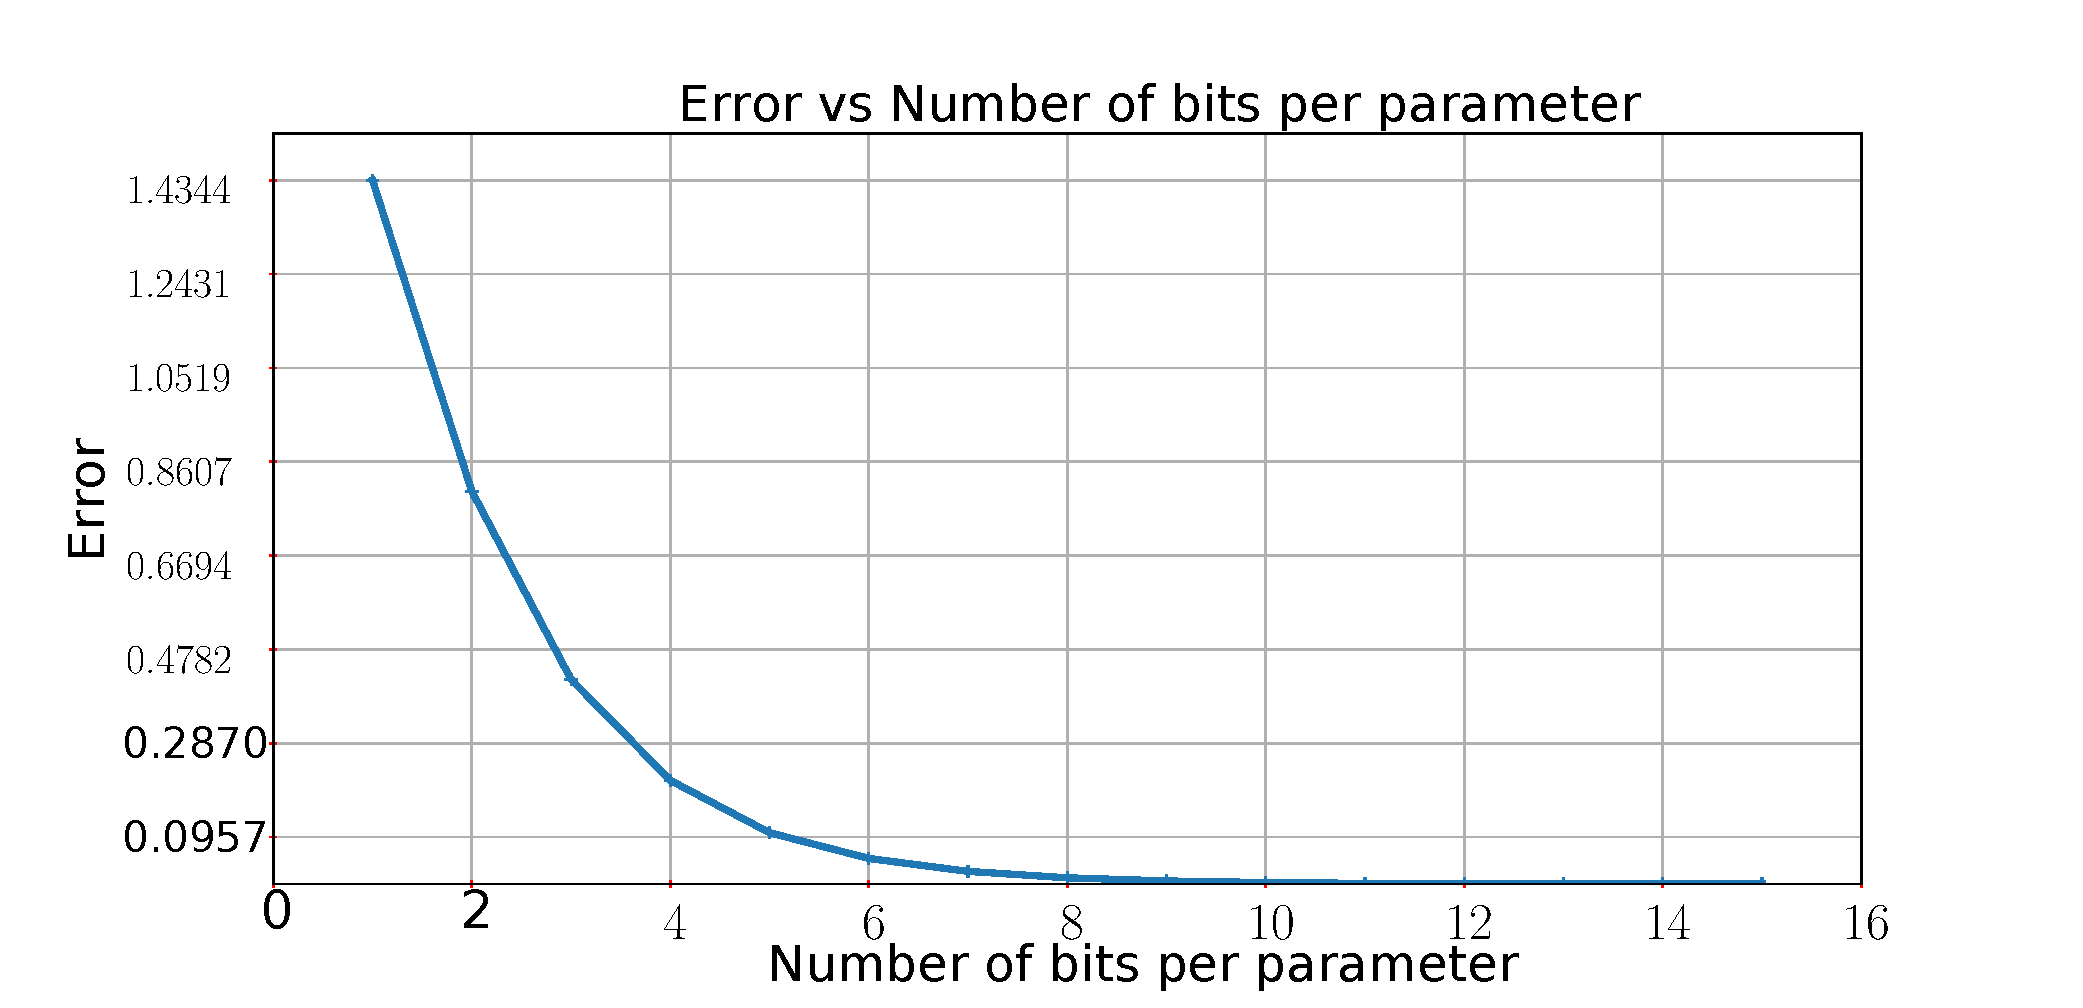
\includegraphics[width=0.5\textwidth]{./figures/bitsvserror}
\caption{\label{err_fig}Error vs bits per parameter}
\end{figure}
$ \bU $ at the transmitter consisting of ten antennas is parameterised and reconstructed  at the receiver with two antennas. So the system as 3 parameters for $\phi_{k_j,j}$ which is uniformly distributed between $(-\pi,\pi]\  \forall k,j$ and 1 parameter for $\theta_{k,l}$ having probability density\cite{roh2004efficient} where k=2 and l=1.
\begin{equation*}
    p(\theta_{k, l})=2l\ \sin^{2l-1}\theta_{k, l}\cos\theta_{k, l}, 0\leq\theta_{k, l} < {\pi\over 2}.
\end{equation*}
in figure ~\ref{err_fig} as the number of bits per parameter is increases the error becomes almost negligible

\begin{figure}[htbp]
\centering
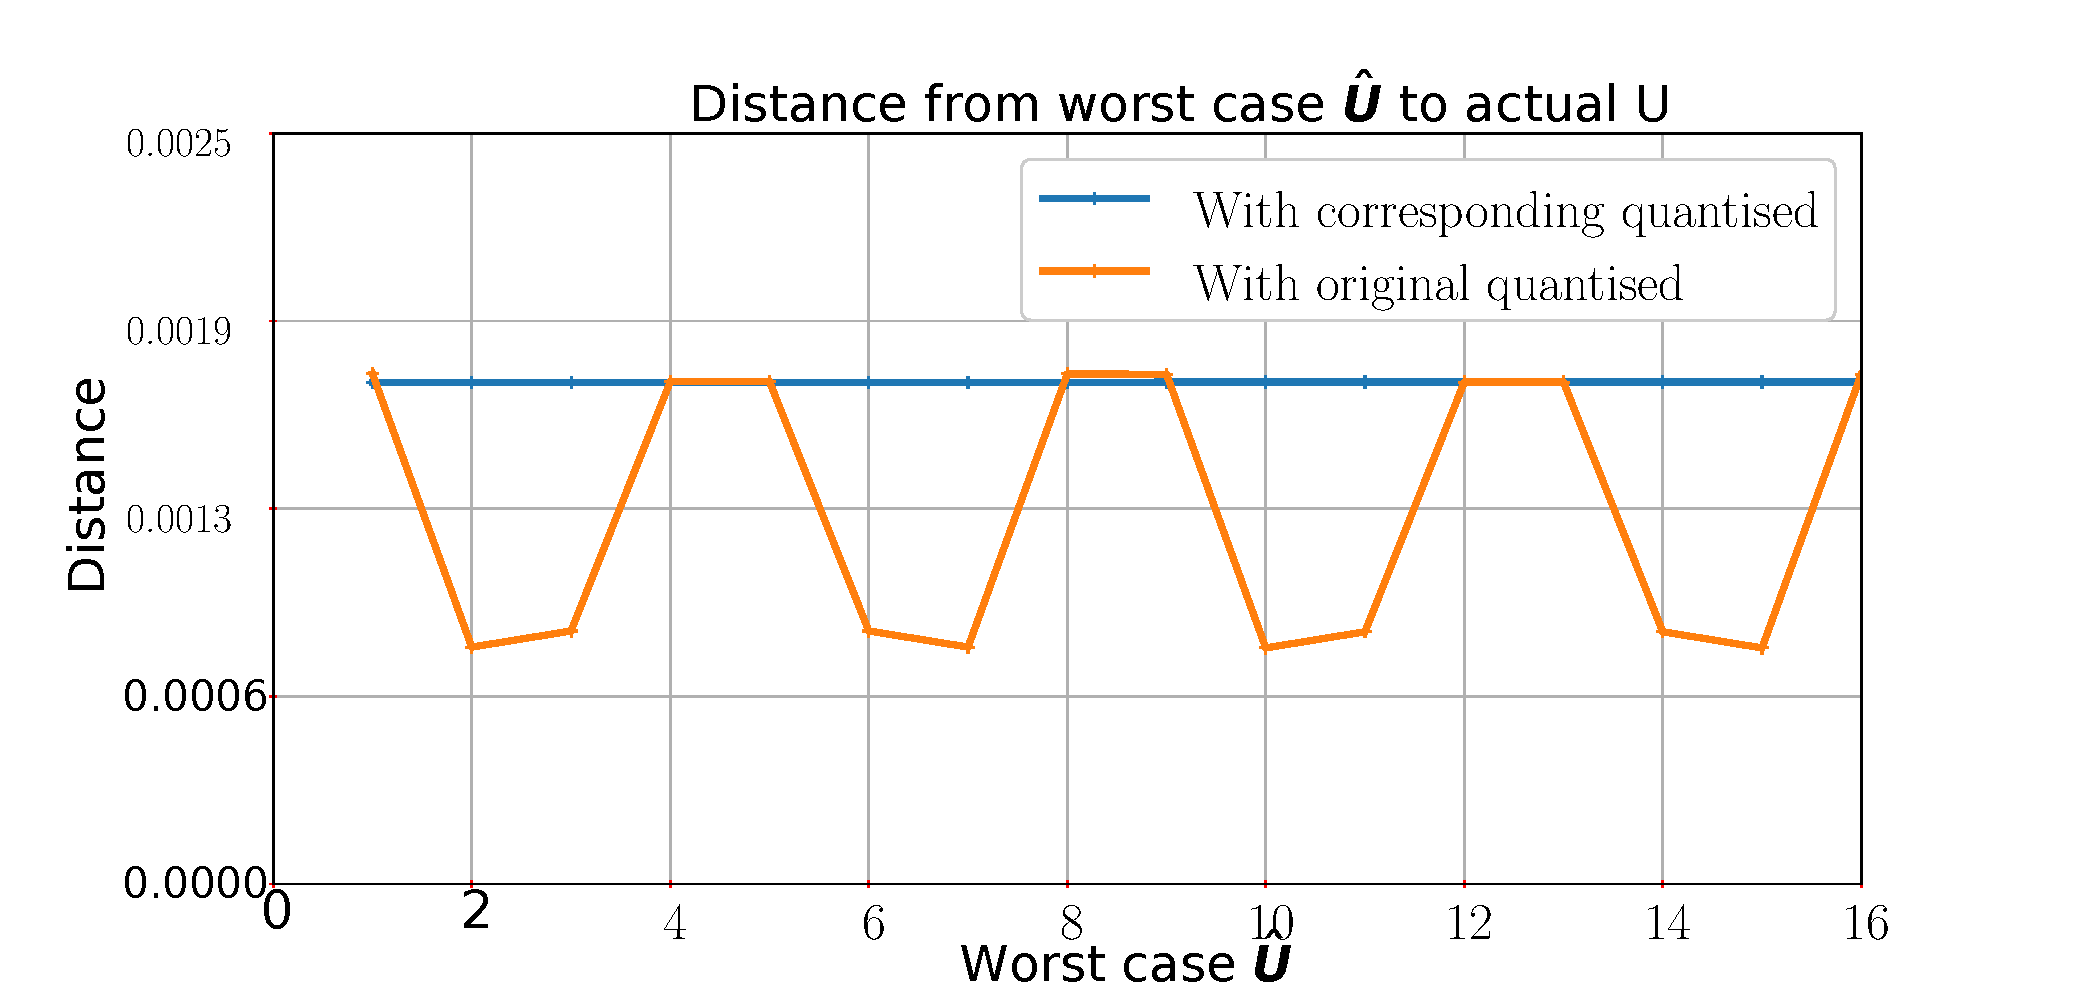
\includegraphics[width=0.5\textwidth]{./figures/u_dist}
\caption{\label{u_dis}Distance from actual $\bU$ to $\hat \bU$}
\end{figure}

\subsection{Achievable rate}
\subsection{BER}


%\section{Conclusion}
\renewcommand{\bibfont}{\footnotesize}
\bibliographystyle{IEEEtran}
\bibliography{IEEEfull,references}

\end{document}
